\chapter{三角方程}
先看下面的实例。

若$E$是$\angle BAC$的角平分线上的一个定点,已知$\angle BAC=60^{\circ}$(图5.1),过$E$点的动直线$BC$交
$\angle BAC$的两边于$B$、$C$. 试问当直线$BC$绕点$E$旋转到什么位置时,$AB=2AC$?

\noindent
\begin{minipage}{.45\textwidth}
\begin{analyze}
当直线旋转时(我们可以用旋转角$x$来刻画这个旋转),$\triangle BAC$是个可变图形。欲使$AB=2AC$,应设法分别找出边$AB$、$AC$与变量$x$的函数关系(这本质上是一个解斜三角形的问题),然后用方程的方法解之.
\end{analyze}
\end{minipage}
\hfill
\begin{minipage}{.45\textwidth}
\centering
\begin{tikzpicture}[scale=.7]
\tkzDefPoints{0/0/A, 4/0/E, 6/0/F}
\tkzDefPoint(-35:3.5){C}
\tkzDefPoint(25:7){B'}
\tkzInterLL(A,B')(C,E)
\tkzGetPoint{B}
\tkzLabelPoints[left](A)
\tkzLabelPoints[below](C,E)
\tkzLabelPoints[above](B)
\draw(B')--(A)--(F);
\tkzDrawPolygon(A,C,B)
\node at (2,0)[below]{$m$};
\tkzMarkAngles[mark=none, size=.8cm](C,A,E F,E,B)
\tkzMarkAngles[mark=none, size=1cm](E,A,B)
\tkzMarkAngles[mark=none, size=.6cm](B,E,A)
\tkzLabelAngle[pos=1.2](F,E,B){$x$}
\tkzLabelAngle[pos=1.1](B,E,A){$180^{\circ}-x$}

\end{tikzpicture}
    \captionof{figure}{}
\end{minipage}

\begin{solution}
由于$E$是$\angle BAC$的角平分线上的定点,故可用字母$m$表示$AE$的长。容易看出$\triangle ABE$是可解的:$\angle BAE=30^{\circ}$, $\angle B=x-30^{\circ}$, $\angle AEB=180^{\circ}-x$,$AE=m$,由正弦定理,得
\[\begin{split}
    \frac{AB}{\sin(180^{\circ}-x)}&=\frac{m}{\sin(x-30^{\circ})}\\
    AB&=\frac{m\sin x}{\sin (x-30^{\circ})}
\end{split}\]
同理,可得:$AC=\frac{m\sin x}{\sin(x+30^{\circ})}$.

欲使$AB=2AC$,应使
\[2m\sin x\sin (x-30^{\circ})=m\sin x\sin(x+30^{\circ})\]
显然$m\sin x\ne 0$,上式可简化为
\[2\sin (x-30^{\circ})=\sin(x+30^{\circ})\]
\end{solution}

这种三角函数符号中含有未知数的等式称为\textbf{三角方程},又如
\[\sin x=\frac{1}{3},\quad \tan^2 x-5\tan x-3=0,\quad 3\cos\frac{x}{2}+\cos x-1=0\]
\[\frac{1+\tan x}{1-\tan x}=1+\sin2x,\quad a\sin x+b\cos x=c,\quad \sin^{100}x+8\sin^5x-2=0\]
等都是三角方程。它们来自数学、物理和技术工程。

本章将研究一些简单三角方程的求解问题。

\section{最简三角方程}
在三角方程中,$\sin x=a$, $\cos x=a$, $\tan x=a$, $\cot x=a$是最简单的(称为\textbf{最简三角方程}),也是最基本的最重要的。其他三角方程的求解,往往是归结为这四种最简三角方程的求解。


\subsection{方程$\sin x=a$的解集}

方程的解集自然依赖于常数$a$的取值和对变元$x$的限定范围。对于后者,若不附任何条件,就意味着是在$(-\infty,+\infty)$上求方程的解集(下同).
\begin{enumerate}[(1)]
    \item 当$|a|>1$时,由于任取$x\in\R$,都有$|\sin x|\le 1$
    
    $\therefore\quad$ 方程无解,即解集为$\emptyset$.
    \item 当$|a|\le 1$时,我们先求出方程的特解(图5.2):
\[\alpha_1=\arcsin a,\qquad \alpha_2=\pi-\arcsin a\]
\begin{figure}[htp]
    \centering
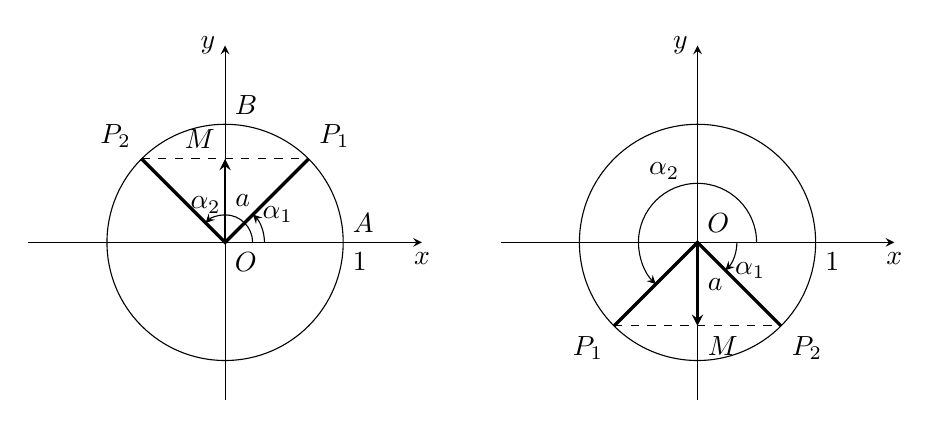
\begin{tikzpicture}[>=stealth]
\begin{scope}
\draw[->](-2.5,0)--(2.5,0)node[below]{$x$};
\draw[->](0,-2)--(0,2.5)node[left]{$y$};
\draw(0,0)node[below right]{$O$} circle (1.5);
\draw[very thick](180-45:1.5)node[above left]{$P_2$}--(0,0)--(45:1.5)node[above right]{$P_1$};
\draw[dashed](180-45:1.5)--(45:1.5);
\draw[thick, ->](0,0)--node[right]{$a$}(0,.75*1.414)node[above left]{$M$};
\draw[->](.5,0) arc (0:45:.5)node[right]{$\alpha_1$};
\draw[->](.35,0) arc (0:135:.35)node[above]{$\alpha_2$};
\node at (1.5,0)[above right]{$A$};
\node at (0,1.5)[above right]{$B$};
\node at (1.5,0)[below right]{$1$};
\end{scope}
\begin{scope}[xshift=6cm]
\draw[->](-2.5,0)--(2.5,0)node[below]{$x$};
\draw[->](0,-2)--(0,2.5)node[left]{$y$};
\draw(0,0)node[above right]{$O$} circle (1.5);
\node at (1.5,0)[below right]{$1$};
\draw[very thick](-135:1.5)node[below left]{$P_1$}--(0,0)--(-45:1.5)node[below right]{$P_2$};
\draw[dashed](-135:1.5)--(-45:1.5);
\draw[thick, ->](0,0)--node[right]{$a$}(0,-.75*1.414)node[below right]{$M$};
\draw[->](.5,0) arc (0:-45:.5)node[right]{$\alpha_1$};
\draw[->](.75,0) arc (0:180+45:.75);
\node at (115:1){$\alpha_2$};

\end{scope}    
\end{tikzpicture}
    \caption{}
\end{figure}
然后,再加上“周期的整数倍”即得到方程的\textbf{通解}:
\[\begin{split}
    x_1&=\arcsin a+2k\pi,\\
    x_2&=(\pi-\arcsin a)+2k\pi,
\end{split}\quad k\in\Z\]
$x_1,x_2$的表达式有时合并写成
\[x=k\pi+(-1)^k\arcsin a,\quad k\in\Z\]
即方程的解集为
\begin{equation}
    \left\{x\mid x=k\pi+(-1)^k\arcsin a,\; k\in\Z\right\}\tag{*}
\end{equation}
\end{enumerate}

应注意:(*)是在$|a|\le 1$时的解集,若忘掉$|a|\le 1$这个条件,说$\sin x=a$的解集是(*),那就不正确.

\subsection{方程$\cos x=a$的解集}
\begin{enumerate}
    \item 当$|a|>1$时,$\cos x=a$的解集为$\emptyset$;
    \item 当$|a|\le 1$时,$\cos x=a$的特解为(图5.3)
\[\alpha_1=\arccos a,\qquad \alpha_2=-\arccos a\]
\begin{figure}[htp]
    \centering
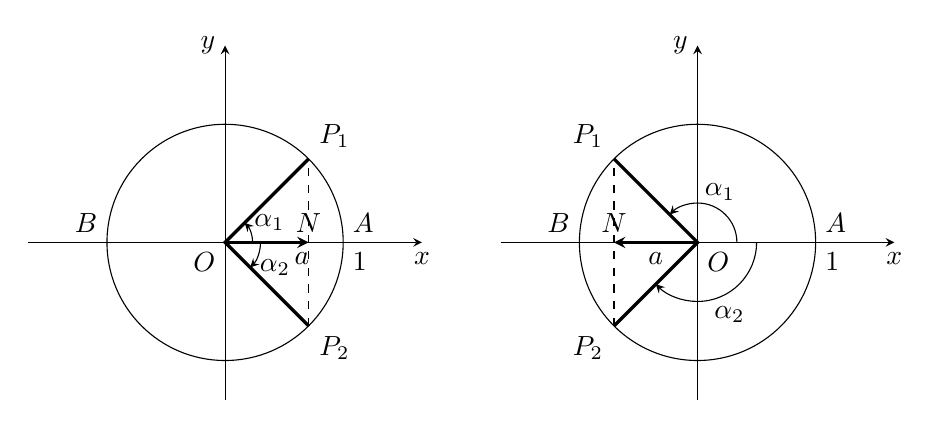
\begin{tikzpicture}[>=stealth]
\begin{scope}
\draw[->](-2.5,0)--(2.5,0)node[below]{$x$};
\draw[->](0,-2)--(0,2.5)node[left]{$y$};
\draw(0,0)node[below left]{$O$} circle (1.5);
\draw[very thick](45:1.5)node[above right]{$P_1$}--(0,0)--(-45:1.5)node[below right]{$P_2$};
\draw[dashed](-45:1.5)--(45:1.5);
\draw[thick, ->](0,0)--(.75*1.414,0)node[above]{$N$};
\node at (.75*1.3,0)[below]{$a$};
\draw[->](.35,0) arc (0:45:.35)node[right]{$\alpha_1$};
\draw[->](.45,0) arc (0:-45:.45)node[right]{$\alpha_2$};
\node at (1.5,0)[above right]{$A$};
\node at (-1.5,0)[above left]{$B$};
\node at (1.5,0)[below right]{$1$};
\end{scope}
\begin{scope}[xshift=6cm]
\draw[->](-2.5,0)--(2.5,0)node[below]{$x$};
\draw[->](0,-2)--(0,2.5)node[left]{$y$};
\draw(0,0)node[below right]{$O$} circle (1.5);
\node at (1.5,0)[above right]{$A$};
\node at (1.5,0)[below right]{$1$};
\draw[very thick](-135:1.5)node[below left]{$P_2$}--(0,0)--(135:1.5)node[above left]{$P_1$};
\draw[dashed](-135:1.5)--(135:1.5);
\draw[thick, ->](0,0)--node[below]{$a$}(-.75*1.414,0)node[above]{$N$};
\draw[->](.5,0) arc (0:135:.5);
\draw[->](.75,0) arc (0:-135:.75);
\node at (-66:1){$\alpha_2$};
\node at (-1.5,0)[above left]{$B$};
\node at (66:.7){$\alpha_1$};
\end{scope}    
\end{tikzpicture}
    \caption{}
\end{figure}


通解为
\[\begin{cases}
    x_1=\arccos a+2k\pi\\
    x_2=-\arccos a+2k\pi
\end{cases} \mathop{\Longleftrightarrow}^{\text{合并为}} x=2k\pi\pm \arccos a,\quad k\in\Z\]
写成解集的形式为
\[\left\{x\mid x=2k\pi\pm\arccos a,\; k\in\Z\right\}\]
\end{enumerate}

\subsection{方程$\tan x=a$的解集}
由于$\tan x$的值域为$(-\infty,+\infty)$,所以对任意$a\in\R$,方程都有解。其特解为(图5.4)
\[\alpha_1=\arctan a,\qquad \alpha_2=\arctan a+\pi\]
其通解为
\[\begin{cases}
    x_1=\arctan a+2k\pi\\
    x_2=(\arctan a+\pi)+2k\pi    
\end{cases}\mathop{\Longleftrightarrow}^{\text{合并为}} x=\arctan a+k\pi,\; k\in\Z  \]
写成解集的形式为$\{x\mid x=\arctan a+k\pi,\; k\in\Z\}$.
\begin{figure}[htp]
    \centering
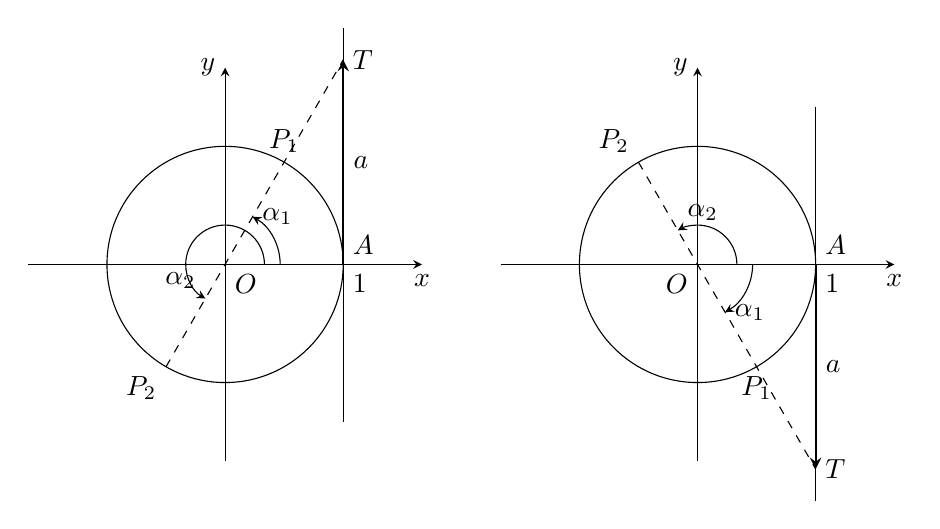
\begin{tikzpicture}[>=stealth]
\begin{scope}
\draw[->](-2.5,0)--(2.5,0)node[below]{$x$};
\draw[->](0,-2.5)--(0,2.5)node[left]{$y$};
\draw(0,0)node[below right]{$O$} circle (1.5);
\draw(1.5,3)--(1.5,-2);
\draw[dashed](-120:1.5)node[below left]{$P_2$}--(60:1.5)node[above]{$P_1$}--(60:3)node[right]{$T$};
\node at (1.5,0)[above right]{$A$};
\node at (1.5,0)[below right]{$1$};
\draw[thick,->](1.5,0)--node[right]{$a$}(60:3);
\draw[->](.5,0) arc (0:180+60:.5)node[above left]{$\alpha_2$};
\draw[->](.7,0) arc (0:60:.7)node[right]{$\alpha_1$};

\end{scope}
\begin{scope}[xshift=6cm]
    \draw[->](-2.5,0)--(2.5,0)node[below]{$x$};
    \draw[->](0,-2.5)--(0,2.5)node[left]{$y$};
    \draw(0,0)node[below left]{$O$} circle (1.5);
    \draw(1.5,2)--(1.5,-3);
    \node at (1.5,0)[above right]{$A$};
    \node at (1.5,0)[below right]{$1$};
    \draw[dashed](120:1.5)node[above left]{$P_2$}--(-60:1.5)node[below]{$P_1$}--(-60:3)node[right]{$T$};
    \draw[thick,->](1.5,0)--node[right]{$a$}(-60:3);
    \draw[->](.5,0) arc (0:120:.5)node[above right]{$\alpha_2$};
    \draw[->](.7,0) arc (0:-60:.7)node[right]{$\alpha_1$};
\end{scope}    
\end{tikzpicture}
    \caption{}
\end{figure}

\subsection{方程$\cot x=a $的解集}

$\cot x$的值域也是$(-\infty,+\infty)$,所以任意$a\in\R$,方程都有解,其特解为(图5.5)
\[\alpha_1=\arccot a,\qquad \alpha_2=\arccot a+\pi\]
其通解为
\[\begin{cases}
    x_1=\arccot a+2k\pi\\
    x_2=(\arccot a+\pi)+2k\pi    
\end{cases}\mathop{\Longleftrightarrow}^{\text{合并为}} x=\arccot a+k\pi,\; k\in\Z  \]
写成解集的形式为$\{x\mid x=\arccot a+k\pi,\; k\in\Z\}$.

\begin{figure}[htp]
    \centering
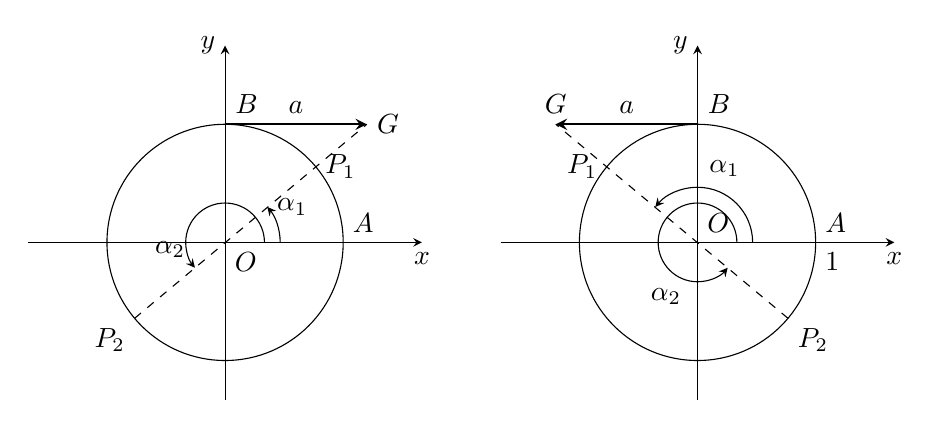
\begin{tikzpicture}[>=stealth]
\begin{scope}
\draw[->](-2.5,0)--(2.5,0)node[below]{$x$};
\draw[->](0,-2)--(0,2.5)node[left]{$y$};
\draw(0,0)node[below right]{$O$} circle (1.5);
\draw[thick, ->](0,1.5)node[above right]{$B$}--node[above]{$a$}(1.2*1.5,1.5)node[right]{$G$};
\draw[dashed](180+40:1.5)node[below left]{$P_2$}--(1.2*1.5,1.5);
\node at (40:1.5)[right]{$P_1$};
\node at (1.5,0)[above right]{$A$};

\draw[->](.5,0) arc (0:180+40:.5)node[above left]{$\alpha_2$};
\draw[->](.7,0) arc (0:40:.7)node[right]{$\alpha_1$};

\end{scope}
\begin{scope}[xshift=6cm]
    \draw[->](-2.5,0)--(2.5,0)node[below]{$x$};
    \draw[->](0,-2)--(0,2.5)node[left]{$y$};
    \draw(0,0)node[above right]{$O$} circle (1.5);
    \draw[thick, ->](0,1.5)node[above right]{$B$}--node[above]{$a$}(-1.2*1.5,1.5)node[above]{$G$};
    \draw[dashed](-40:1.5)node[below right]{$P_2$}--(-1.2*1.5,1.5);
    \node at (180-40:1.5)[left]{$P_1$};
    \node at (1.5,0)[above right]{$A$};
    \node at (1.5,0)[below right]{$1$};
    \draw[->](.5,0) arc (0:270+50:.5);
    \draw[->](.7,0) arc (0:180-40:.7);
    \node at (70:1){$\alpha_1$};
    \node at (-120:.8){$\alpha_2$};

\end{scope}    
\end{tikzpicture}
    \caption{}
\end{figure}

\begin{example}
    解方程:
\begin{multicols}{3}
\begin{enumerate}[(1)]
    \item $2\sin x+\sqrt{2}=0$
    \item $2\cos 2x=1$
    \item $\tan(x+15^{\circ})+1=0$
\end{enumerate}
\end{multicols}
\end{example}

\begin{solution}
\begin{enumerate}
    \item $2\sin x+\sqrt{2}=0\Longleftrightarrow \sin x=-\frac{\sqrt{2}}{2}$
\[\begin{split}
    \therefore\quad x_1&=\arcsin\left(-\frac{\sqrt{2}}{2}\right)+2k\pi=-\frac{\pi}{4}+2k\pi\\
    x_2&=\pi-\arcsin\left(-\frac{\sqrt{2}}{2}\right)+2k\pi=\frac{5\pi}{4}+2k\pi\\
\end{split}\qquad (k\in\Z)\]
写成解集\footnote{求方程解集的过程叫解方程. 为了书写简便,也可以只列出所有的解而不必写成集合形式.}为
\[\left\{x\mid x=-\frac{\pi}{4}+2k\pi \text{ 或 } x=\frac{5\pi}{4}+_2k\pi,\; k\in\Z\right\}\]

\item $2\cos 2x=1\Longleftrightarrow \cos 2x=\frac{1}{2}$

$\therefore\quad 2x=2k\pi\pm \arccos\frac{1}{2} \quad \Rightarrow\quad x=k\pi\pm\frac{\pi}{6}\quad (k\in\Z) $

写成解集为$\left\{x\mid x=k\pi\pm \frac{\pi}{6},\; k\in\Z\right\}$

\begin{rmk}
下面的解法是错误的:
\[2x=\pm \arccos\frac{1}{2},\qquad x=\pm\frac{1}{2} \arccos \frac{1}{2}\]
$\therefore\quad x=2k\pi\pm \frac{1}{2} \arccos \frac{1}{2}\quad (k\in\Z)$.
\end{rmk}


\item $\tan(x+15^{\circ})+1=0 \Longleftrightarrow \tan (x+15^{\circ})=-1$,

$\therefore\quad (x+15^{\circ})=\arctan(-1)+k\cdot 180^{\circ}=-45^{\circ}+180^{\circ}\cdot k$

$\therefore\quad x=-60^{\circ}+180^{\circ}\cdot k\quad (k\in\Z)$.

写成解集为$\{x\mid x=-60^{\circ}+180^{\circ}\cdot k,\;  k\in\Z\}$。

\begin{rmk}
    在同一个表达式中应使用相同的单位。
    
    如上面的式子不能写成$x+15^{\circ}=-\frac{\pi}{4}+k\pi\; (k\in\Z)$的形式。
\end{rmk}
\end{enumerate}
\end{solution}


\begin{example}
    若$0^{\circ}<x<360^{\circ}$,解方程$\sin(3x-105^{\circ})=-\frac{1}{2}$.
\end{example}

\begin{solution}
\[\begin{split}
\because\quad &(3x_1-105^{\circ})=\arcsin\frac{1}{2}+360^{\circ}\cdot k=30^{\circ}+360^{\circ}\cdot k\quad (k\in\Z)   \\
&(3x_2-105^{\circ})=180^{\circ}-\arcsin\frac{1}{2}+360^{\circ}\cdot k=150^{\circ}+360^{\circ}\cdot k\quad (k\in\Z)   
\end{split}\]

$\therefore\quad x_1=45^{\circ}+120\cdot k,\qquad x_2=85^{\circ}+120^{\circ}\cdot k\quad (k\in\Z)$

考虑到$0^{\circ}<x<360^{\circ}$,
\begin{enumerate}
    \item 在$x_1$中令$k=0,1,2$,得$45^{\circ},\; 165^{\circ},\; 285^{\circ}$;
    \item 在$x_2$中令$k=0,1,2$,得$85^{\circ},\; 205^{\circ},\; 325^{\circ}$.
\end{enumerate}

$\therefore\quad $原方程的解集为$\{45^{\circ},\; 165^{\circ},\; 285^{\circ},\; 85^{\circ},\; 205^{\circ},\; 325^{\circ}\}$.
\end{solution}

\section*{习题一}
\begin{center}
    \bfseries A
\end{center}
\begin{enumerate}
    \item 口答下列方程的解集:
\begin{multicols}{3}
\begin{enumerate}[(1)]
    \item $\sin x=\frac{\sqrt{3}}{2}$
    \item $\sin x=-\frac{1}{2}$
    \item $\cos x=\frac{\sqrt{2}}{2}$
    \item $\cos x=-\frac{1}{2}$
    \item $\tan x=-\sqrt{3}$
    \item $\cot x=\frac{1}{3}$
\end{enumerate}
\end{multicols}
    \item 解下列方程:
  \begin{multicols}{2}
\begin{enumerate}[(1)]
    \item $2\sin2x+1=0$
    \item $\sin\left(\frac{x}{2}+\frac{\pi}{6}\right)=\frac{\sqrt{3}}{2}$
    \item $2\cos\left(\frac{\pi}{3}+45^{\circ}\right)=1$
    \item $\tan 2x-\sqrt{3}=0$
    \item $\frac{1}{2}\cot 2(x+25^{\circ})-2=0$
    \item $3\tan\frac{x+20^{\circ}}{3}=\sqrt{3}$ 
    
$(-1000^{\circ}<x<1000^{\circ})$
\end{enumerate}
\end{multicols}
\end{enumerate}

\section{简单三角方程}
一些简单的三角方程,可以通过三角函数的恒等变形或代数方法,化归上节研究过的四种最简三角方程,从而获得其解。现举几类,着重说明“化归”的思路和方法,悟出了道理,可见一般。

\subsection{同角同名的三角函数方程}
\begin{example}
   解下列方程: 
\begin{multicols}{2}
\begin{enumerate}[(1)]
    \item $2\sin^2 x-5\sin x-3=0$
    \item $\sin^2 x-\cos^2 x=\cos x$
    \item $3\cos\frac{x}{2}+\cos x=1$
    \item $\frac{1+\tan x}{1-\tan x}=1+\sin 2x$
\end{enumerate}
\end{multicols}
\end{example}

\begin{analyze}
把新问题化归为已研究过的问题,是数学研究中的通法。对于(1),实行换元,即令$\sin x=y$,可得到关于$y$的一元二次方程,从而可以解出$y$,这就化归为最简 三角方程的第一种。其余几题,只须稍作三角函数变换,就可以实现化归。
\end{analyze}

\begin{solution}
\begin{enumerate}[(1)]
    \item 令$y=\sin x\; (-1\le y\le 1)$,有$2y^2-5y-3=0$,即$$(y-3)(2y+1)=0\Rightarrow y_1=3,\; y_2=\frac{-1}{2}$$

$\therefore\quad \sin x=3$(无解);$\sin x=\frac{-1}{2}$ 解之,得
\[x_1=\frac{-\pi}{6}+2k\pi,\quad x_2=\frac{7\pi}{6}+2k\pi,\; k\in\Z\]
\item 把$\sin x$化为$\cos x$,得
\[2\cos^2x+\cos x-1=0\]
令$\cos x=y\; (-1\le y\le 1)$,有$2y^2+y-2=0$,
即$$(y+1)(2y-1)=0\Longleftrightarrow y_1=-1,\quad y_2=\frac{1}{2}$$
\[\begin{split}
    \therefore\quad \cos x=-1 &\Longleftrightarrow x_1=\pi+2k\pi \; (k\in\Z)\\
    \cos x=\frac{1}{2}&\Longleftrightarrow x_2=2k\pi \pm \frac{\pi}{3}\; (k\in\Z)
\end{split}\]
\item 把$\cos x$写成 $2\cos^2\frac x2-1$, 可得
$$2\cos ^{2}\frac x2+ 3\cos \frac x2- 2= 0$$
令$y=\cos\frac{x}{2}\quad (-1\leqslant y\leqslant1)$, 有
$$2y^{2}+ 3y- 2= 0\Longleftrightarrow y_{1}= - 2,\quad y_{2}= \frac 12$$
即 $\cos \frac x2= - 2$ (无解),\quad $\cos\frac x2=\frac12$

$\therefore\quad \frac x2= 2k\pi \pm$ $\frac \pi 3\left ( k\in Z\right ) \Longleftrightarrow x= 4k\pi \pm \frac {2\pi }3\left ( k\in Z\right ) $

\item 把$\sin2x$写成$\frac{2\tan x}{1+\tan ^{2}x}$, 有$\frac {1+ \tan x}{1- \tan x}= 1+ \frac {2\tan x}{1+ \tan ^{2}x}$,

令 $y= \tan x$, 有
\[\begin{split}
    \frac {1+ y}{1- y}- 1= \frac {2y}{1+ y^{2}}&\Longleftrightarrow \frac {2y}{1- y}- \frac {2y}{1+ y^{2}}= 0\\
    &\Longleftrightarrow 2y\left(\frac{1}{1-y}-\frac{1}{1+y^{2}}\right)=0\\
    &\Longleftrightarrow 2y\cdot\frac{y(y+1)}{(1+y^{2})(1-y)}=0\\
    &\Longleftrightarrow y_{1}= 0,\quad y_{2}= - 1
\end{split}\]
即 
\[\begin{split}
    \tan x= 0&\Longleftrightarrow x_1= k\pi\quad ( k\in \Z) \\
    \tan x= -1&\Longleftrightarrow x_{2}= - \frac \pi 4+ k\pi\quad ( k\in \Z) 
\end{split}\]
\end{enumerate}
\end{solution}

\begin{remark}
    此例的特点和化归方法可以简捷地概括为“同角同名(包括可化为同角同名函数的方程)——换元就行”。此例中,每小题都列出了所有的解,而未写成解集的形式。
\end{remark}

\subsection{两同名函数相等的方程}

这类方程的一般形式为
\begin{align}
    \sin f(x)&=\sin g(x) \tag{1}\\
    \cos f(x)&=\cos g(x) \tag{2}\\
    \tan f(x)&=\tan g(x) \tag{3}\\
    \cot f(x)&=\cot g(x) \tag{4}
\end{align}

对于(1),可把$g(x)$看作是$f(x)$的特解(图5.6),有
\[\begin{split}
 f(x)&=g(x)+2k\pi\; (k\in\Z)\longrightarrow \text{解出}x_1\\
f(x)&=\pi-g(x)+2k\pi\; (k\in\Z)\longrightarrow \text{解出}x_2
\end{split}\]
则方程(1)的解集为$\{x\mid x=x_1\text{ 或 }x=x_2\}$;

\noindent
\begin{minipage}{.45\textwidth}
    \centering
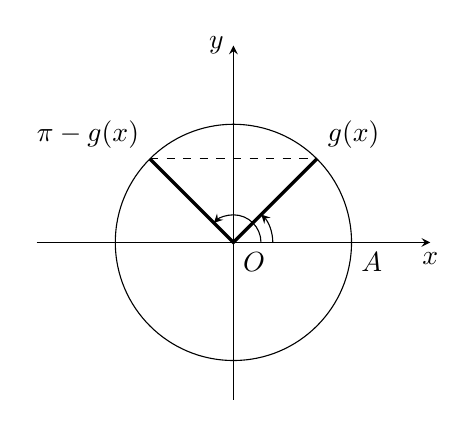
\begin{tikzpicture}[>=stealth]
\draw[->](-2.5,0)--(2.5,0)node[below]{$x$} ;   
\draw[->](0,-2)--(0,2.5)node[left]{$y$} ;   
\draw(0,0)node[below right]{$O$} circle (1.5);
\draw[very thick](135:1.5)node[above left]{$\pi-g(x)$}--(0,0)--(45:1.5)node[above right]{$g(x)$};
\draw[dashed](135:1.5)--(45:1.5);
\draw[->](.5,0) arc (0:45:.5);
\draw[->](.35,0) arc (0:135:.35);
\node at (1.5,0)[below right]{$A$};
\end{tikzpicture}    
\captionof{figure}{}
\end{minipage}\hfill
\begin{minipage}{.45\textwidth}
    \centering
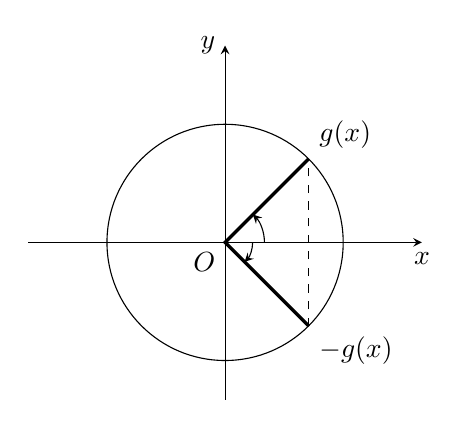
\begin{tikzpicture}[>=stealth]
    \draw[->](-2.5,0)--(2.5,0)node[below]{$x$} ;   
\draw[->](0,-2)--(0,2.5)node[left]{$y$} ;   
\draw(0,0)node[below left]{$O$} circle (1.5);
\draw[very thick](-45:1.5)node[below right]{$-g(x)$}--(0,0)--(45:1.5)node[above right]{$g(x)$};
\draw[dashed](-45:1.5)--(45:1.5);
\draw[->](.5,0) arc (0:45:.5);
\draw[->](.35,0) arc (0:-45:.35);
\end{tikzpicture}    
\captionof{figure}{}
\end{minipage}

对于(2),仍然把$g(x)$看作是$f(x)$的特解(图5.7),有
\[ f(x)=2k\pi\pm g(x)\; (k\in\Z)\longrightarrow \text{由此解出}x_1,x_2\]
则方程(2)的解集为$\{x\mid x=x_1\text{ 或 }x=x_2\}$;

同样,对于(3)有$f(x)=g(x)+k\pi\; (k\in\Z)\longrightarrow \text{由此解出}x$;

对于(4)有$f(x)=g(x)+k\pi\; (k\in\Z)\longrightarrow \text{由此解出}x$.

\begin{example}
解方程:
\begin{multicols}{2}
\begin{enumerate}[(1)]
    \item $\tan 4x=\tan 3x$
    \item $\sin4x+\sin2x=0$
\end{enumerate}
\end{multicols}
\end{example}

\begin{solution}
\begin{enumerate}[(1)]
    \item 由$\tan 4x=\tan 3x$得:$4x+3x+k\pi\; (k\in\Z)$

$\therefore\quad x=k\pi\; (k\in\Z)$
\item 由题可得:$\sin 4x=\sin(-2x)$

$\therefore\quad 4x=(-2x)+2k\pi\; (k\in\Z)$,或$4x=\pi-(-2x)+2k\pi\; (k\in\Z)$,有
\[\begin{split}
    6x=2k\pi,&\qquad 2x=\pi+2k\pi\\
x_1=\frac{k\pi}{3}\; (k\in\Z) &\qquad x_2=\frac{\pi}{2}+k\pi \; (k\in\Z)
\end{split}\]

$\therefore\quad $原方程的解集为$\left\{x\mid x=\frac{k\pi}{3}\text{ 或 }x=\frac{\pi}{2}+k\pi,\; k\in\Z\right\}$.
 \end{enumerate}   
\end{solution}

\section*{习题二}
\begin{center}
    \bfseries A
\end{center}

解下列方程:
\begin{enumerate}
    \item $2\sin^{2}x+3\sin x+1=0$
    \item $4\sin^{2}x+(2\sqrt{3}-2)\cos x-(4-\sqrt{3})=0$
\begin{multicols}{2}
    \item $\sec^{2}x=1+\tan x$
    \item $\cos2\theta-\cos3\theta=0$
    \item $\sin3x+\sin4x=0$
    \item $\cot x+\cot3x=0$
    \item $\cos2x+\sin3x=0$
    \item $\sin x=2\sin\left(\frac{\pi}{3}-x\right)$    
\end{multicols}
\end{enumerate}

\subsection{左边化积(分解因式化积或和差化积)右边方程}

从代数上我们知道,方程
$F(x)=f_1(x)\cdot f_2(x)=0$
在函数的定义域$Q$上[不妨把$Q$也称为方程$F(x)=0$的定义域],若$f_1(x)=0$和$f_2(x)=0$的解集分别是$A$与$B$,那么$F(x)
=0$的解集就是$A\cup B$,即
\[F(x)=0,\; x\in Q \Longleftrightarrow f_1(x)=0,\; x\in Q\text{\;与\;}f_2(x)=0,\; x\in Q\]

这里应该特别注意方程$f_1(x)=0$,$f_2(x)=0$是在$Q$上求解,如果忽略了$x\in Q$这个前提,就可能导致错误。


\begin{example}
    解方程:
    \begin{multicols}{2}
\begin{enumerate}[(1)]
    \item $\sin x\cdot \tan x\cdot \cot x=0$
    \item $\sin x\cdot \tan x\cdot \sec x=0$
\end{enumerate}        
    \end{multicols}
\end{example}

\begin{solution}
\begin{enumerate}[(1)]
    \item 方程的定义域为$Q:x\in\R$,且$x\ne \frac{\pi}{2}+k\pi,\; x\ne k\pi\; (k\in\Z)$。显然,在$Q$上$\sin x\ne 0$,$\tan x\ne 0$,$\cot x\ne 0$
    
    $\therefore\quad $原方程无解(或说解集为$\emptyset$)。
\item 方程的定义域为$Q:x\in\R$,且$x\ne \frac{\pi}{2}+k\pi\; (k\in\Z)$。
\[\begin{split}
    \therefore\quad \sin x=0\; (x\in Q)&\Longleftrightarrow x_1=k\pi\; (k\in\Z)\\
    \tan x=0\; (x\in Q)&\Longleftrightarrow x_2=k\pi\; (k\in\Z)\\
  \sec  x=0\; (x\in Q)&\Longleftrightarrow  \frac{1}{\cos x}=0\; (x\in Q) \Longleftrightarrow x\in\emptyset\\
\end{split}\]
\end{enumerate}

$\therefore\quad $原方程的解为$x=k\pi\; (k\in\Z)$.
\end{solution}

\begin{thm}
{思考题} 对于$\sin x\cdot \cot x=0$,下述解法为什么不正确?

由$\sin x\cdot \cot x=0$得
\[\sin x=0\Longleftrightarrow x_1=k\pi\; (k\in\Z)\]
或
\[\cot x=0\Longleftrightarrow x_2=\frac{\pi}{2}+k\pi\; (k\in\Z)\]
$\therefore\quad $原方程的解为$x_1$与$x_2$.
\end{thm}

\begin{example}
    解方程$\sin4x+\sin2x=0$.
\end{example}

\begin{solution}
\textbf{解法1:}左边分解因式化积,$$2\sin2x\cos2x+\sin2x=0\Longleftrightarrow \sin2x(2\cos2x+1)=0$$
其定义域为$Q:x\in\R$(当$Q=\R$时,有时可略去不写),则
\[\begin{split}
    \sin2x=0,\quad &\text{或}\quad 2\cos2x+1=0\\
    2x=k\pi\; (k\in\Z),\quad &\text{或}\quad 2x=2k\pi \pm \frac{2\pi}{3}\; (k\in\Z)\\
    x_1=\frac{k\pi}{2}\; (k\in\Z),\quad &\text{或}\quad x_2=k\pi \pm \frac{\pi}{3}\; (k\in\Z)\\   
\end{split}\]

$\therefore\quad $原方程的解为$x_1,x_2$

\textbf{解法2:}左边和差化积,得
\[2\sin3x\cdot \cos x=0 \Longleftrightarrow \sin3x=0\quad \text{或}\quad \cos x=0\]
\[3x=k\pi \; (k\in\Z ),\qquad x_2=2k\pi \pm \frac{\pi}{2}\; (k\in\Z )\]

$x_1=\frac{k\pi}{3}\; (k\in\Z)$;($x_2$也可写成$\frac{\pi}{2}+k\pi\; (k\in\Z )$)

$\therefore\quad $原方程的解为$x_1,x_2$.

\textbf{解法3:}原方程为$\sin4x=sin(-2x)$,
\[\begin{split}
 4x=(-2x)+2k\pi ,\quad &\text{或}\quad 4x=\pi -(-2x)+2k\pi \\
6x=2k\pi ,\quad &\text{或}\quad 2x=\pi +2k\pi    
\end{split}\]
$\therefore\quad x_1=\frac{k\pi}{3}\; (k\in\Z );\quad x_2=\frac{\pi}{2} +k\pi\; (k\in\Z )$.

这里,应该注意:由于解法不同,解在形式上可能有差
异。如方法1与方法2的结果虽然形式不同。我们分别在图5.8与图5.9上标出解法1与解法2的结果发现,两种方法得到的\textbf{解集实质上相同}(利用代数上证明两个集合相等的方法可以作出证明).
    
\noindent
\begin{minipage}{.45\textwidth}
\centering
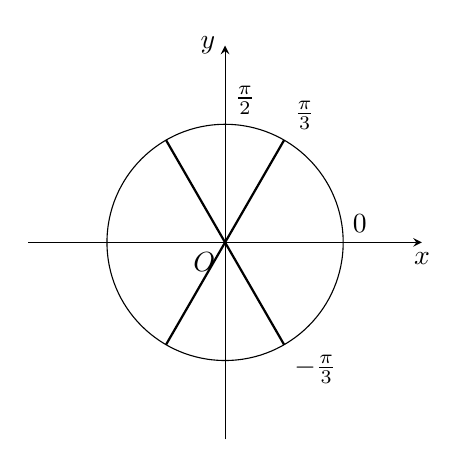
\begin{tikzpicture}[>=stealth]
\draw[->](-2.5,0)--(2.5,0)node[below]{$x$};
\draw[->](0,-2.5)--(0,2.5)node[left]{$y$};
\draw(0,0)node [below left]{$O$}circle(1.5);
\foreach \x in {0,60,90,120,180,-60,-120,-90}
{
    \tkzDrawPoint(\x:1.5)
}
\draw[thick](-60:1.5)node[below right]{$-\frac{\pi}{3}$}--(120:1.5);
\draw[thick](60:1.5)node[above right]{$\frac{\pi}{3}$}--(-120:1.5);
\node at (1.5,0)[above right]{0};
\node at (0,1.5)[above right]{$\frac{\pi}{2}$};

\end{tikzpicture}
\captionof{figure}{}
\end{minipage}
\hfill
\begin{minipage}{.45\textwidth}
    \centering
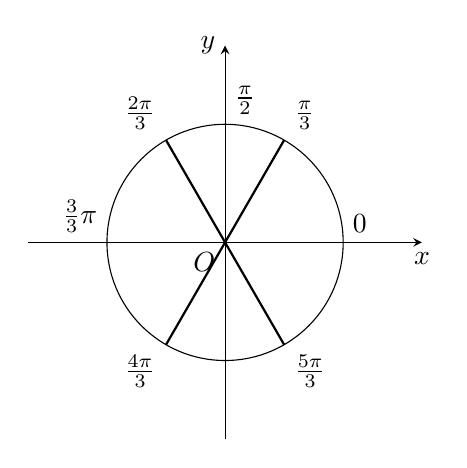
\begin{tikzpicture}[>=stealth]
\draw[->](-2.5,0)--(2.5,0)node[below]{$x$};
\draw[->](0,-2.5)--(0,2.5)node[left]{$y$};
\draw(0,0)node [below left]{$O$}circle(1.5);
\foreach \x in {0,60,90,120,180,-60,-120,-90}
{
    \tkzDrawPoint(\x:1.5)
}
\draw[thick](-60:1.5)node[below right]{$\frac{5\pi}{3}$}--(120:1.5)node[above left]{$\frac{2\pi}{3}$};
\draw[thick](60:1.5)node[above right]{$\frac{\pi}{3}$}--(-120:1.5)node[below left]{$\frac{4\pi}{3}$};
\node at (1.5,0)[above right]{0};
\node at (0,1.5)[above right]{$\frac{\pi}{2}$};
\node at (-1.5,0)[above left]{$\frac{3}{3}\pi$};

\end{tikzpicture}
\captionof{figure}{}
\end{minipage}
\end{solution}

\begin{example}
    解方程:$\sin x\cos x+1=\sin x+\cos x$
\end{example}

\begin{solution}
\textbf{解法1:}原方程即
\[(\cos x-1)(\sin x-1)=0\]
\[\begin{split}
\cos x-1=0,\quad &\text{或}\quad \sin x-1=0\\
\cos x=1,\quad &\text{或}\quad \sin x=1\\
x_1=2k\pi\; (k\in\Z ),\quad &\text{或}\quad x_2=\frac{\pi}{2}+2k\pi\; (k\in\Z )
\end{split}\]
$\therefore\quad $方程的解为$x_1$、$x_2$.

\textbf{解法2:}令$y=\sin x+\cos x$,则$y^2=1+2\sin x\cos x$

$\therefore\quad \sin x\cos x=\frac{y^2-1}{2}$,
代入原方程,得$y^2-2y+1=0$,
\[(y-1)^2=0\Longleftrightarrow y=1\]
即
\[\sin x+\cos x=1 \Longleftrightarrow \sqrt{2}\sin\left(x+\frac{\pi}{4}\right)=1 \Longleftrightarrow \sin\left(x+\frac{\pi}{4}\right)=\frac{1}{\sqrt{2}}\]
其解为
\[x+\frac{\pi}{4}=\frac{\pi}{4}+2k\pi\; (k\in\Z)\Longleftrightarrow x_1=2k\pi\; (k\in\Z)\]
或
\[x+\frac{\pi}{4}=\frac{3\pi}{4}+2k\pi\; (k\in\Z)\Longleftrightarrow x_2=\frac{\pi}{2}+2k\pi\; (k\in\Z)\]
$\therefore\quad $原方程的解为$x_1$、$x_2$.
\end{solution}

\begin{example}
    解方程:$\frac{\sin2x}{\cos x}=\frac{\cos2x}{\sin x}$
\end{example}

\begin{solution}
\textbf{解法1:}原方程$\Longleftrightarrow \frac{\sin2x}{\cos x}-\frac{\cos 2x}{\sin x}=0$
,即
\[\begin{split}
\frac{-\cos 3x}{\sin x\cos x}&=0\Longleftrightarrow \begin{cases}
    \cos3x=0 \Leftrightarrow \cos x(4\cos^2 x-3)=0\\
    \sin x\cos x\ne 0   
\end{cases} 
\\
&\Longleftrightarrow \cos^2 x=\frac{3}{4}\Longleftrightarrow \cos x=\pm\frac{\sqrt{3}}{2} \qquad \text{(图5.10)}
\end{split} \]
$\therefore\quad x=\pm\frac{\pi}{6}+k\pi\; (k\in\Z)$

\noindent
\begin{minipage}{.45\textwidth}
    \centering
\begin{tikzpicture}[>=stealth]
\draw[->](-2.5,0)--(2.5,0)node[below]{$x$};
\draw[->](0,-2)--(0,2)node[left]{$y$};
\draw(0,0)node [below left]{$O$}circle(1.5);
\draw[very thick](30:1.5)node[right]{$\frac{\pi}{6}$}--(-150:1.5);
\draw[very thick](-30:1.5)node[right]{$-\frac{\pi}{6}$}--(150:1.5);
\foreach \x in {30,150}
{
    \draw[dashed](\x:1.5)--(-\x:1.5);
}
\node at (1.3,0)[above left]{$N$};
\node at (-1.3,0)[above right]{$N'$};
\node at (1.3,0)[below]{$\tfrac{\sqrt{3}}{2}$};
\node at (-1.3,0)[below]{$-\tfrac{\sqrt{3}}{2}$};

\end{tikzpicture}
\captionof{figure}{}
\end{minipage}
\hfill
\begin{minipage}{.45\textwidth}
\begin{remark}
这里我们运用了一系列同解变形的步骤(关键的是哪几步?),这就保证了最后得到的$x$是原不等式的解。下面的解法先去分母(会增解呢?还是丢解?你能讲清楚解方程时增解或丢解的最根本原由吗?)。
\end{remark}
\end{minipage}

\textbf{解法2:}去分母,得$\sin2x\sin x-\cos2x\cos x=0$,即$-\cos3x=0$,

$\therefore\quad 3x=\frac{\pi}{2}+k\pi\; (k\in\Z)\Longleftrightarrow x=\frac{\pi}{6}+\frac{k\pi}{3}\; (k\in\Z)$.

在单位圆上可以看得出,这里得到的解实际上可以写成$x_1=\pm\frac{\pi}{6}+k\pi\; (k\in\Z )$与$x_2=\frac{\pi}{2}+k\pi\; (k\in\Z )$. 代入原方程可知$x_2$是增根,所以$x_1$是原方程的解。

\begin{remark}
    这里,产生增根的原因是:“去分母”这一步扩大了方程的定义域(因而,去分母不是同解变形),所以产生了增根.
\end{remark}
\end{solution}

在解三角方程中,若出现了增(减)根,处理起来往往很不容易。因此,避免出现增(减)根——也就是注意步步要使用同解变形
——可能是最佳选择。这时根本的原则是“保证方程的定义域既不扩大,也不缩小”。

\section*{习题三}
\begin{center}
    \bfseries A
\end{center}

解下列方程:
\begin{enumerate}
    \item $\sin2x-\sqrt{2} \cos x=0$
    \item $\sin2x+\sqrt{3}\sin x-6\cos x -3\sqrt{3}=0$
    \begin{multicols}{2}
    \item $\cos2x=\cos x+\sin x$
    \item $\sin x=\cos\frac{x}{2}$
    \item $\sin3x-\sin5x=0$
    \item $\cos2x-\cos x=0$
    \item $\tan 4x=\tan 2x$
    \item $\sin3x+\cos2x=0$
\end{multicols}
\end{enumerate}


\begin{center}
    \bfseries B
\end{center}
\begin{multicols}{2}
\begin{enumerate}\setcounter{enumi}{8}
    \item $\sin x+\sin 2x+\sin 3x=0$
    \item $\tan x+\tan 2x+\tan 3x=0$
\end{enumerate}
\end{multicols}

\subsection{正弦、余弦的齐次方程}
从代数上我们知道,下列方程:
\[\begin{split}
&ax+by=0\qquad \text{($a$、$b$不同时为零)}\\
&ax^2+bxy+cy^2=0\qquad \text{($a$、$b$、$c$不同时为零)}\\
&ax^3+bx^2y+cxy^2+dy^3=0\qquad \text{($a$、$b$、$c$、$d$不同时为零)}
\end{split}\]
都是关于$x$、$y$的$n$次齐次方程(要特别注意右边为零)。若同时以$\sin x$、$\cos x$分别去代替上述方程中的$x$、$y$,就得到了关于$\sin x$、$\cos x$的$n$次$(n\in\N)$齐次方程(各项系数不全为零):
\[\begin{split}
&  a\sin x+b\cos x=0\\
&a\sin^2x+b\sin x\cos x+c\cos^2x=0\\
&a\sin^3x+b\sin^2x\cos x+c\sin x\cos^2x+d\cos^3x=0
\end{split}\]

以下,研究这类方程的解法。


\begin{example}
    解下列方程:
\begin{enumerate}[(1)]
    \item $5\sin x+2\cos x=0$
\item $2\sin2x+3\sin x\cos x+\cos^2x=0$
\item $3\sin^2x-4\sin x\cos x+5\cos^2x=2$
\end{enumerate}
\end{example}

\begin{solution}
\begin{enumerate}[(1)]
    \item $\because\quad \cos x=0$的解不是原方程的解,方程两边同除以$\cos x$,得
 \[ 5\tan x+2=0\Longleftrightarrow \tan x=-\frac{2}{5}\]

$\therefore\quad x=\arctan\left(-\frac{2}{5}\right)+k\pi\quad (k\in\Z)$

\item $\because\quad \cos x=0$的解不是原方程的解,方程两边同除以$\cos^2 x$,得
\[2\tan^2 x+3\tan x+1=0\]
\[\tan x=-1\quad \text{或}\quad \tan x=-\frac{1}{2}\]
\[\begin{split}
    x_1&=-\frac{\pi}{4}+k\pi \; (k\in\Z)\\
    x_2&=\arctan\left(-\frac{1}{2}\right)+k\pi =-\arctan \frac{1}{2}+k\pi \; (k\in\Z)\\
\end{split}\]
从而:$x_1,x_2$都是原方程的解.

\item 原方程可以写成
\[\begin{split}
    3\sin^2 x-&4\sin x\cos x+5\cos^2 x=2(\sin^2x+\cos^2 x)\\
    &\Longleftrightarrow \sin^2x-4\sin x\cos x+3\cos^2 x=0
\end{split} \]
(这就化归为齐次方程了)

$\because\quad \cos x=0$的解不是原方程的解,方程两边同除以$\cos^2 x$,得
\[\tan^2 x-4\tan x+3=0\]
由此$\tan x=3$或$\tan x=-1$,
\[\begin{split}
    x_1&=\arctan3+k\pi \quad  (k\in\Z)\\
    x_2&=\frac{\pi}{4}+k\pi \quad  (k\in\Z)
\end{split}\]
$\therefore\quad$原方程的解为$x_1,x_2$.
\end{enumerate}    
\end{solution}

\begin{remark}
    关于$\sin x$、$\cos x$的$n$次齐次方程,都可以通过两边同除以$\cos^n x$化成只含$\tan x$的方程,从而即可获解.
\end{remark}

\subsection{正弦、余弦的一次方程}
关于正弦、余弦的一次方程
\begin{equation}
    a\sin x\pm b\cos x=c\quad (a,b\ne 0) \tag{*}
\end{equation}
根据2.6节的和差化积公式,引入辅助角$\varphi$(图5.11)(*)可化为
\[r(\sin x\cos\varphi\pm\cos x\sin\varphi)=c\quad \left(r=\sqrt{a^2+b^2}\right)\]
即
\[\sin(x\pm\varphi)=\frac{c}{\sqrt{a^2+b^2}}\]
这就实现了“化归”. 

\noindent
\begin{minipage}{.45\textwidth}
    \centering
\begin{tikzpicture}[>=stealth]
\draw[->](-1.5,0)--(2.5,0)node[below]{$x$};
\draw[->](0,-1.5)--(0,2.5)node[left]{$y$};
\draw[very thick](0,0)node[below left]{$O$}--node[left]{$r$}(0.833,2)node[right]{$P(a,b)$};
\draw[->](.5,0) arc (0:67.8:.5)node[right=2mm]{$\varphi$};
\end{tikzpicture}
\captionof{figure}{}
\end{minipage}
\hfill
\begin{minipage}{.45\textwidth}
    \centering
\begin{tikzpicture}[>=stealth]
\draw[->](-1.5,0)--(2.5,0)node[below]{$x$};
\draw[->](0,-1.5)--(0,2.5)node[left]{$y$};
\draw[very thick](0,0)node[below left]{$O$}--node[left]{$r$}(0.833,2)node[right]{$P(5,12)$};
\draw[->](.5,0) arc (0:67.8:.5)node[right=2mm]{$\varphi$};
\end{tikzpicture}
\captionof{figure}{}
\end{minipage}

\begin{example}
解下列方程:
\begin{multicols}{2}
\begin{enumerate}[(1)]
    \item $5\sin x-12\cos x=6.5$
    \item $6\cos x-8\sin x=9$
\end{enumerate}
\end{multicols}
\end{example}

\begin{solution}
\begin{enumerate}[(1)]
    \item 如图5.12,$r=\sqrt{5^2+12^2}=13$,原方程可化为
\[13\left(\sin x\cdot \frac{5}{13}-\cos x\cdot \frac{12}{13}\right)=\frac{13}{2}\]

$\therefore\quad \sin(x-\varphi)=\frac{1}{2}$,$\varphi$为锐角,且$\tan\varphi=\frac{12}{5}$

\[x-\varphi=\frac{\pi}{6}+2k\pi\; (k\in\Z)\quad \text{或}\quad x-\varphi=\frac{5\pi}{6}+2k\pi\; (k\in\Z)\]

$\therefore\quad x_1=\frac{\pi}{6}+\arctan\frac{12}{5}+2k\pi,\quad x_2=\frac{5\pi}{6}+\arctan\frac{12}{5}+2k\pi\; (k\in\Z) $

$\therefore\quad $原方程的解为$x_1,x_2$.

\item $8\sin x-6\cos x=-9,\quad r=\sqrt{8^2+6^2}=10$

$\therefore\quad \sin(x-\varphi)=-\frac{9}{10}$,$\varphi$为锐角,且$\tan\varphi=\frac{3}{4}$
\[x-\varphi=\arcsin\left(-\frac{9}{10}\right)+2k\pi\; (k\in\Z) \]
或\[x-\varphi=\pi-\arcsin\left(-\frac{9}{10}\right)+2k\pi\; (k\in\Z) \]
\[\begin{split}
    \therefore\quad x_1&=-\arcsin\frac{9}{10}+\arctan\frac{3}{4}+2k\pi\; (k\in\Z)\\
    x_2&=\pi+\arcsin\frac{9}{10}+\arctan\frac{3}{4}+2k\pi\; (k\in\Z)\\
\end{split}\]
$\therefore\quad $原方程的解为$x_1,x_2$.
\end{enumerate}
\end{solution}

\begin{rmk}
在解的表达式中,若反三角函数的值为特殊角,都必须表成特殊角的形式。   
\end{rmk}

\section*{习题四}
\begin{center}
    \bfseries A
\end{center}

\begin{enumerate}
    \item 在下列$x$、$y$的齐次方程中(设$x\ne 0$)能求出$\frac{y}{x}$吗?试试看:
\begin{multicols}{2}
    \begin{enumerate}[(1)]
        \item $3x-5y=0$
        \item $6x^2+7xy-3y^2=0$
        \item $x^3-4x^2y-xy^2+5y^3=0$
    \end{enumerate}    
\end{multicols}

\item 解下列方程:
\begin{enumerate}[(1)]
    \item $2\sin x-\sqrt{3}\cos x=0$
    \item $3\sin x=\sqrt{3}\cos x$
    \item $5\cos 2x+2\sin2x=0$
    \item $2\sin^2 x+3\sin x\cos x+\cos^2x=0$
    \item $2\sin^{2}x=4\cos^{2}x-7\sin x\cos x$
    \item $\cos^{2}x+\frac{2\sqrt{3}}{3}\sin x\cos x-\sin^{2}x=0$
    \item $5\sin^{2}x+7\sin x\cos x+4\cos^{2}x=1$
    \item $6\sin^{2}x+3\sin x\cos x-5\cos^{2}x=2$
    \item $3\sin^{2}x-\sin2x-\cos^{2}x=0$
    \item $\cos2x+3\sin2x+4\sin^{2}x+1=0$
\end{enumerate}

\item 解下列方程:
\begin{multicols}{2}
\begin{enumerate}[(1)]
\item $\sin x+\cos x=1$
\item $\sin x+\sqrt{3}\cos x=1$
\item $2\sin x+7\cos x=6$
\item $3\cos x-4\sin x+2=0$
\item $\sqrt{5}\cos 3x-2\sin 3x-3=0$
\end{enumerate}    
\end{multicols}
\end{enumerate}


\section{本章小结}

\subsection{知识结构分析}
\begin{center}
\begin{tikzpicture}[>=stealth]
\node[draw] (A) at (-4.5,0)[text width=2.4cm, align=center]{(四种)\\最简三角方程\\的解集};
\node[draw] (B) at (0,0)[text width=2.4cm, align=center]{(五类)\\简单三角方程\\的解法};
\node[draw] (C) at (4.5,0)[text width=2.4cm, align=center]{(其余)\\简单三角方程\\的解法};
\draw[->](B)--node[text width=2cm, align=center]{求解方向\\化归}(A);
\draw[->](C)--node[text width=2cm, align=center]{求解方向\\化归}(B);
\node[draw] (D) at (0,2)[text width=4.5cm, align=center]{三角方程的\\定义、特解与解集(通解)};
\draw[decorate, decoration={brace, amplitude=10pt}](-5,1)--(5,1);
\end{tikzpicture}
\end{center}


\subsection{几点说明}
\begin{enumerate}
\item 四种最简方程是解三角方程的基础,也是求三角方程解的“化归”方向。其解集应掌握得十分熟练;
\item 解简单三角方程的基本思想是“化归”(按结构图中箭头指示的方向进行),即化为已经解决或易于解决的问题。这是数学中经常运用的思想方法。
\item 对于五类简单三角方程也应熟记其模式和求解方法。
\end{enumerate}

以下补充几例,进一步说明之。


\begin{example}
解方程:$8\sin^2\frac{x}{2}+3\sin x-4=0$
\end{example}

\begin{solution}
\textbf{解法1:}
\[8\cdot \frac{1-\cos x}{2}+3\sin x-4=0\Longleftrightarrow 3\sin x-4\cos x=0\]
(这是正、余弦的齐次方程)

$\therefore\quad \tan x=\frac{4}{3},\quad x=\arctan\frac{4}{3}+k\pi\; (k\in\Z)$

\textbf{解法2:}
\[8\sin^2\frac{x}{2}+6\sin\frac{x}{2}\cos\frac{x}{2}-4\left(\sin^2\frac{x}{2}+\cos^2\frac{x}{2}\right)=0\]
即:
\[\begin{split}
    4\sin^2\frac{x}{2}+6\sin\frac{x}{2}\cos\frac{x}{2}-4\cos^2\frac{x}{2}&=0\\
    2\sin^2\frac{x}{2}+3\sin\frac{x}{2}\cos\frac{x}{2}-2\cos^2\frac{x}{2}&=0
\end{split}\]
(这是正、余弦的齐次方程)

\[\begin{split}
\therefore\quad 2\tan^2\frac{x}{2}+3\tan\frac{x}{2}-2&=0 \\
\left(2\tan\frac{x}{2}-1\right)\left(\tan\frac{x}{2}+2\right)&=0\\
\tan\frac{x}{2}=\frac{1}{2}\quad &\text{或}\quad \tan\frac{x}{2}=-2\\
\frac{x}{2}=\arctan\frac{1}{2}+k\pi\quad &\text{或}\quad \frac{x}{2}=\arctan(-2)+k\pi
\end{split}\]

$\therefore\quad x_1=2\arctan\frac{1}{2}+2k\pi\quad \text{或}\quad x_2=2\arctan(-2)+2k\pi\; (k\in\Z)$
\end{solution}

\begin{example}
解方程:$\cos^3 x-\cos x\sin x-\sin^3 x=1$
\end{example}

\begin{solution}
$(\cos^3 x-\sin^3 x)-\cos x\sin x-1=0$
\[\begin{split}
&(\cos x-\sin x)(\cos^2 x+\cos x\sin x+\sin^2 x)-(\cos x\sin x+1)=0\\
&(\cos x\sin x+1)(\cos x-\sin x-1)=0
\end{split}\]
\[\begin{split}
    \therefore\quad \frac{1}{2}\sin 2x+1=0&\quad \text{或}\quad \sin x-\cos x=-1\\
    \sin2x=-2\text{(无解)}&\qquad \sin\left(x-\frac{\pi}{4}\right)=\frac{-1}{\sqrt{2}}\\
\end{split}\]
\[\begin{split}
x-\frac{\pi}{4}=-\frac{\pi}{4}+2k\pi&\quad \text{或}\quad x-\frac{\pi}{4}=\frac{5\pi}{4}+2k\pi\; (k\in\Z)\\
x_1=2k\pi &\quad \text{或}\quad  x_2=\frac{3\pi}{2}+2k\pi\; (k\in\Z)
\end{split}\]

$\therefore\quad $原方程的解是$x_1$与$x_2$.
\end{solution}

\begin{example}
求方程$|2\sin^2 x-1|-\cos x=0$的解集.
\end{example}

\begin{solution}
利用$\cos2x=1-2\sin^2 x$,得:
\[|2\sin^2 x-1|=|-\cos 2x|=|\cos2x|\]
原方程变为
\[|\cos 2x|=\cos x\Longleftrightarrow \begin{cases}
    \cos x\ge 0 & (1)\\
    \cos 2x=\pm \cos x &(2)
\end{cases}\]
\begin{enumerate}
    \item 对于$\cos 2x=\cos x$,$2x=2k\pi\pm x\; (k\in\Z)$

$\therefore\quad x_1=2k\pi, \quad x_2=\frac{2}{3}k\pi\; (k\in\Z)$

$\because\quad x$不满足(1),舍去. $x_1$是原方程的解.

\item 对于$\cos 2x=-\cos x$,可得:$2\cos^2 x+\cos x-1=0$

\[\cos x=\frac{1}{2}\quad \text{或}\quad \cos x=-1\; \text{(不满足(1),舍去)}\]

$\therefore\quad x=2k\pi\pm \frac{\pi}{3}\; (k\in\Z)$
\end{enumerate}

综上,原方程的解集为$\left\{x\mid x=2k\pi\text{ 或 }x=2k\pi\pm\frac{\pi}{3},\; k\in\Z\right\}$
\end{solution}


\section*{复习题五}
\begin{center}
    \bfseries A
\end{center}

\begin{enumerate}
    \item 解下列方程:
\begin{enumerate}[(1)]
    \begin{multicols}{2}
    \item $6\sin^2 2x=\sin 4x+3$
    \item $3\sin 2x-9\cos x+2\sin x=3$        
    \end{multicols}
\end{enumerate}

\item 解下列方程:
\begin{enumerate}[(1)]
\begin{multicols}{2}
    \item $\sin x=2\sin\left(\frac{\pi}{3}-x\right)$
    \item $\sin\left(x+\frac{\pi}{6}\right)+\cos\left(x+\frac{\pi}{6}\right)=0$    
\end{multicols}
    \item $\sin\left(2x+\frac{\pi}{3}\right)+\sin\left(x-\frac{\pi}{6}\right)=0$
    \item $\cos\left(x+\frac{\pi}{4}\right)+\sec\left(x+\frac{\pi}{4}\right)+2=0$
    \item $\sin\left(x+\frac{\pi}{4}\right)\cdot \sin\left(x-\frac{\pi}{12}\right)=\frac{1}{2}$   
\begin{multicols}{2}
    \item $\sin^{4}x-\cos^{4}x=\cos x+\sin x$
    \item $\cos2\theta=\cos\theta+\sin\theta$    
\end{multicols}

\end{enumerate}

\item 解下列方程:
\begin{enumerate}[(1)]
\begin{multicols}{2}
    \item $\sin6x\cos x=\sin4x\cos3x$
    \item $\sin x\sin7x=\sin3x\sin5x$
    \item $\sin5\theta-\sin3\theta=\sqrt{2}\cos4\theta$
    \item $\sin7\theta-\sin3\theta=\sin\theta$    
\end{multicols}
\end{enumerate}

\item 求证:
\begin{enumerate}[(1)]
\item 方程$\sin^2x=\sin^2\alpha$的解集是$\{x\mid x=k\pi\pm\alpha,\; k\in \Z\}$ 
\item 方程$\cos^2x=\cos^2\alpha$的解集是$\left\{x\mid x=k\pi\pm \alpha,\; k\in\Z\right\}$
\item 方程$\tan^{4}x=\tan^{2}\alpha$的解集是$\{x\mid x=k\pi\pm \alpha,\; k\in \Z\}$
\end{enumerate}

\noindent
\begin{minipage}{.6\textwidth}
\item 如图有一块正方形钢板,一个角上有伤痕,要把它截成
一块正方形钢板,面积是原钢板的$\frac{2}{3}$, 应按怎样的角
度$x$来截?

\item 解下列方程:
\begin{enumerate}[(1)]
    \item $\frac{\cos2x}{1-\sin2x}=0$
    \item $\frac{\sin3x}{\sin2x}=\frac{\cos3x}{\cos2x}$
    \item $\frac{1-\cos2x}{2\cos x}=\frac{\sin2x}{1-\cos2x}$
    \item $\tan\left(\frac{\pi}{3}+x\right)+\tan\left(\frac{\pi}{6}-x\right)=\frac{4}{\sqrt{3}}$
\end{enumerate}
\end{minipage}
\hfill
\begin{minipage}{.5\textwidth}
\centering
\begin{tikzpicture}[>=stealth, scale=.85]
\draw[thick](0,0) rectangle (4,4);
\draw[very thick](3,0)--node[left]{$b$}(4,3)--(1,4)--(0,1)--cycle;
\node at (1.5,0)[below]{$n$};
\node at (3.5,0)[below]{$m$};
\node at (2,4)[above]{$a$};
\draw[pattern=north east lines](.5,4) arc (0:-41:2)--(0,4)--(.5,4);
\draw(3.25,0) arc (0:71.6:.25)node[right]{$x$};

\end{tikzpicture}
\captionof*{figure}{(第5题)}
\end{minipage}

\end{enumerate}

\begin{center}
    \bfseries B
\end{center}

\begin{enumerate}\setcounter{enumi}{6}
\item 方程$\cos2x+\sin x+q=0$,当$q$满足什么条件时才有解?
\item 设$0\leqslant\alpha<\beta\leqslant\pi$, 问$\alpha$、$\beta$为何值时下式的值与$\theta$无关:
$$F(\theta)=\sin^2\theta+\sin^2(\theta+\alpha)+\sin^2(\theta+\beta) $$
\item 解方程$\arctan x+2\arctan\frac1x=\frac{2\pi}3$
\item 解方程$\cos^2x+\cos^2 3x=1$
\item 解不等式$\arcsin(1-x)+\arcsin(1-x^{2})<0$ 
\item (选择题)若$0<\varphi<\frac\pi2$, 则下列各式中成立的是\hfill(\qquad)
\begin{enumerate}[(A)]
    \item $\arcsin(\cos\varphi)>\arccos(\sin\varphi)$
    \item $\arcsin(\cos\varphi)<\arccos(\sin\varphi)$
    \item $\arcsin(\cos\varphi)=\arccos(\sin\varphi)$
    \item 大小关系由$\varphi$的大小而定。
\end{enumerate}
\end{enumerate}
